% Example use of document class for research/technical/research review reports
% at CTU FIT (http://fit.cvut.cz)
% 2015/04/12 Created by Ondrej Guth <ondrej.guth@fit.cvut.cz>



% Nutno napsat v souladu s metodickym pokynem pro vydavani 
% vyzkumnych, souhrnnych a technickych zprav na FIT CVUT




% % % % 
% OPTIONS of the class
% LANGUAGE:
% czech 
% english
% TYPE
% research
% technical
% review
% FONT NORMALSIZE
% 10pt
% 11pt
% 12pt
% % 
\documentclass[english,technical,10pt]{FITreport}[2018/01/26]

\usepackage[utf8]{inputenc}

\usepackage{lmodern} % unicode version of Computer Modern font
\usepackage{amsthm}
% \usepackage{hyperref}

% % % % % 
% Use ALL of the following commands
% % % % % 

\title{The State-of-the-Art of Automated Testing of Models of Cyber-Physical Systems\thanks{The research has been supported by SGS grant No. SGS17/213/OHK3/3T/18}}
\author{Tomáš Apeltauer\thanks{The author would like to express his gratitude for intellectual support, ideas and feedback, to his supervisor doc. Dipl.-Ing. Dr. techn. Stefan Ratschan.}\affil{Department of Digital Design\\\theFIT}
	}
\abstractL{We are presenting a State-of-the-Art that anchors our research in the world of the complex systems, it's models, combination of physical continuous environment with discrete computation environment, testing and verifications according to a specifications and requirements, etc. We look on a problem of automated testing from a different points of view and discuss, whether current methods and approaches are sufficent, or if they present a challenge that can be overcome. We are presenting the goal of our research and propose a direction that we believe will lead to a new, more succesful and better optimized methods.}
%\abstractEN{Abstract in English (used only with reports written in Czech).}
\keywordsL{cyber-physical systems, model-based design, metric temporal logic, model testing and verification, Simulink, hardware-In-The-Loop, embedded computers, simulation of models, automotive}
%\keywordsEN{list of keywords in English (used only with reports written in Czech).}
\reportNumber{02}
\reportYear{18}
\published{January 2018}

% % % % % % % % % % 

\begin{document}

\theoremstyle{definition}
\newtheorem{lemma}{Lemma}
\newtheorem{theorem}[lemma]{Theorem}
\newtheorem{definition}[lemma]{Definition}
\newtheorem{preposition}[lemma]{Preposition}
\newtheorem{example}[lemma]{Example}
\newtheorem{corollary}[lemma]{Corollary}
\newtheorem{proposition}[lemma]{Proposition}
\newtheorem{property}[lemma]{Property}
\newtheorem{observation}[lemma]{Observation}
\theoremstyle{remark}
\newtheorem{notation}[lemma]{Notation}
\newtheorem{note}[lemma]{Note}




\section{Introduction}

In the last decade we have seen a dramatic decrease in the cost of certain computation technologies and such phenomenon gave a birth of a new family of embedded control systems that are much better prepared for fluent, realistic interaction with the continuous physical world around them. For systems that combine physical world around us with the world of cybernetics, we use a term cyber-physical system.

In addition new communication technologies and protocols have been established so all these devices have the potential to be a part of a grid that can grow at very fast rate. All these new options are bringing up many challenges for engineers and academics, because we do not yet have a mature science to support systems engineering of high-confidence cyber-physical systems \cite{NSF:CPS:2017}.

\section{Cyber-physical systems}

The concept of a cyber-physical system is a generalization of embedded systems. An embedded system consists of hardware and software integrated within a mechanical or and electrical system designed for a specific purpose. The term cyber-physical system is a buzzword  nowadays and it is not easy to define it. Take these three definitions from different academic sources.

\begin{definition}[Cyber-physical systems]
    Represents transformative technologies for managing interconnected systems between its physical assets and computational capabilities \cite{LEE201518}.
\end{definition}

\begin{definition}[Cyber-physical systems]
    Refers to a new generation of systems with integrated computational and physical capabilities that can interact with humans through many new modalities \cite{Baheti:2011}.

\end{definition}

\begin{definition}[Cyber-physical systems]
    Are physical and engineered systems whose operations are monitored, coordinated, controlled and integrated by a computing and communication core \cite{Rajkumar:2010}.

\end{definition}

\begin{definition}\label{def:Rajeev}[Cyber-physical systems]
    Consist of a collection of computing devices communicating with one another and interacting with the physical world via sensors and actuators in a feedback loop \cite{Alur:2015:PCS:2774947}.
\end{definition}

In this paper, we will be assuming that the most suitable definition is ~\ref{def:Rajeev}. Cyber-physical system (CPS) consists of a controller computational unit, sensors, actuators and a physical world around it which system must observe and interact with. CPS are reactive systems which react on surrounding environment in an ongoing manner. There is an endless loop of data collection and input evaluation throughout the time. In a cyber-physical system, the controller consists of a discrete software, concurrent components operating in multiple modes of operation, interacting with the continuously evolving physical environment.

\subsection{Motivation for using cyber-physical systems}

Advance in the field of cyber-physical systems will bring us closer to usage of high-speed, low-cost, and real-time embedded computers in technologies like electric networks that employ advanced monitoring \cite{Xue:2016}, networked autonomous vehicles \cite{Lee:2008} or prosthesis as neural controlled artificial leg \cite{Zhang:2012}. CPS are a research priority for both, government agencies (National Science foundation) \cite{NSF:CPS:2017} and industry (automotive, avionics, medical devices).

\subsection{Challenges in the area of cyber-physical systems}

In comparison to the traditional software development architecture, the creation of control software for CPS differs in the emphasis on the security, confidence, reliability and performance of the system. An automotive car that would occasionally bumb into obstacles, or did not stop before junction when the red ligh is on, is probably not going to be very popular among people. CPS are intended to operate in areas which have direct impact on people’s lives and carry much more responsibility than now widely used systems.

High safety and reliability requirements can be particularly difficult if we consider that CPS are interacting mainly with the continuous physical and unpredictable world. Such environment puts many obstacles in a development of the final product.

In the world of embedded systems engineers put a lot of requirements for high reliability and predictability both on the hardware and software. For CPS these requirements will only get more strict. CPS are intended to be deployed in areas as automotive industry, avionics or medical devices. Apart from embedded systems, CPS will not be operating in a controlled environments and must be robust to handle unexpected conditions and adapt to a subsystem failures \cite{Lee:2008}.

\subsubsection{Real-time computing}
CPS are intended to seamlessly interact with the physical world around and thus in an infinite feedback loop. Computations in CPS computation unit are affected by the data gathered from sensors and based on the result of the outcome, the system reacts accordingly. Such real-time computing can be very challenging, because it usually consist of processing huge amount of inputs and delivering immediate reactions. Life-cycle of a creation of such complex system usually contains simulations, either of the whole system, or only part of it. When simulating the system partially using a prototype of our control unit, we call this approach a Hardware-in-the-Loop. Part of the system is already created, while the other part is being real-time simulated \cite{Usenmez:2009}.

\subsubsection{Concurrence}

When defining CPS, many publications emphasize the importance of concurrency. Communication and data exchange is indeed an important part of CPS, but not a necessity. Many CPS are based on a distributed network model or combines together multiple devices into one, more compact system. Since there are not yet mature techniques for the development of a solid, purely concurrent, real-time software, science has to respond appropriately and create such techniques \cite{Lee:2008}.

\section{Models of cyber-physical systems}

The design of a complex cyber-physical system — especially one with heterogeneous subsystems distributed across networks — is a demanding task. Commonly employed design techniques are sophisticated and include mathematical modeling of physical systems, formal models of computation, simulation of heterogeneous systems, software synthesis, verification, validation, and testing \cite{Jensen:2011}.

\subsection{Model-Based design}

Embedded system is usually constructed from the physical plant and the controller module. The controller contains specific algorithm, designed for capabilities and resources of a given embedded system. In the industry production area a Model-driven development paradigm has been deployed and successfully adopted for the development of the embedded systems. Unfortunately when we move from simple programs to a more complex software systems and particularly to a cyber-physical systems, former design techniques and tools are no longer applicable.

A different paradigm was created, founded on a Model-based design. Jensen et al. \cite{Jensen:2011} propose a 10-step methodology for developing cyber-physical systems:

\begin{enumerate}
\item State the Problem
\item Model Physical Processes
\item Characterize the Problem
\item Derive a Control Algorithm
\item Select Models of Computation
\item Specify Hardware
\item Simulate
\item Construct
\item Synthesize Software
\item Verify, and Validate, and Test
\end{enumerate}

This approach helps designers break enormous task of the creation of CPS into manageable iterations, which can be repeated if needed, or to which we can return if we identify an error. Using such paradigm we can create a whole model of the CPS by moving forward through a set of steps that can address at first general and later more concrete aspects of the cyber-physical system. As soon as we have the model complete this methodology helps us to specify and create a real prototype that we can further test and verify.

\subsection{Model-Based V shaped design process}

The traditional design process of the development of the power electronics was based on four simple steps:

\begin{enumerate}
\item Specification of the system
\item Design of the system
\item Implementation of the system
\item Testing and verification
\end{enumerate}

Which inevitably led to a creation of a prototype which was later used for testing and verification phases. This approach had many disadvantages, for example if an engineer discovered and error in a specification, the whole process of the development had to be repeated. In some cases, creation of a prototype is costly and perhaps even impossible, so this methodology could not be used. Implementation was usually manually coded and any design changes, or updates meant a modification at the code level, which can be costly depending on the circumstances.

\begin{figure}
\centering
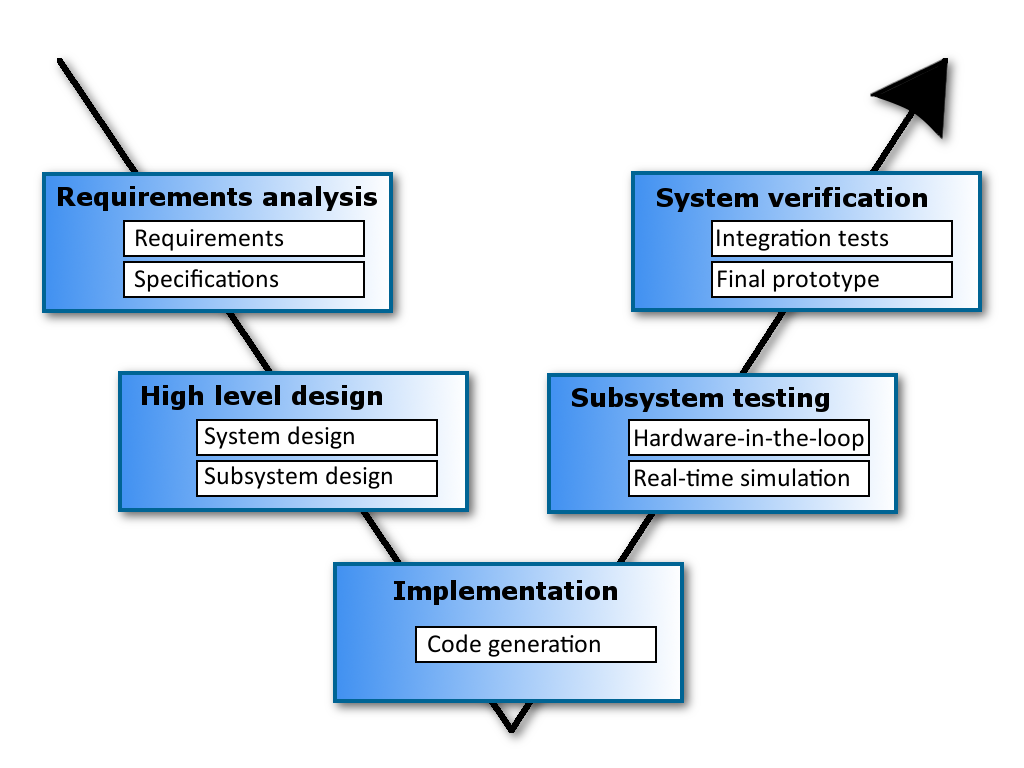
\includegraphics[scale=0.35]{pictures/model_based_design_Vcycle.png}
\caption{The V-cycle of Model-Based design process}
\label{fig:modelBasedDesignProcess}
\end{figure}

That is why a Model-Based design pattern was created and deployed in practise (see fig. \ref{fig:modelBasedDesignProcess}). Model-Based design overcomes obstacles of the traditional design process by unification of all phases of the development cycle into one place, represented by a model. Whole process is centered around a mathematical model of the desired system. This method is usually shown as V shaped design process. Starting by specifications and requirements we are practically describing a mathematical model of a system and such formal specifications can be verified, tested and optimized. Following design phase then fluently moves the model creation to another dimension with the usage of model design tools like Matlab/Simulink/Stateflow, Ptolemy or SystemModeler. The sub-component and component models are being created here.

Testing and verification of a model is non-trivial and although there exist plenty of tools and algorithms to achieve model correctness assurance (an example can be S-Taliro tools) this is still an active area of research. Big advantage of a model-based design is the possibility to real-time simulate desired system and debug the model. After all corrections are done, final model is used to generate the code which rapidly accelerate the whole development process. In the next phases we test the model against hardware by Hardware-in-the-Loop simulation and verify the system from the integration point of view by integration tests. This whole pattern helps us to discover any design flaws in an early stage of the development and enables us to quickly redesign the model if needed.

\subsection{Example of a model of cyber-physical system}

As an example of model of a cyber-physical system can be used an experimental electro-mechanical brake model with disk wiping \cite{Oehlerking:2015}. In their case study Strathmann and Oehlerking present a simplified model of electro-mechanical brake and three verification tools that were tested on the model. Model consists of a plant and a controller.

\section{Model Verification and testing}

During model-based design process we gather clearer and more concrete representation of the desired system but in addition at each phase we are able to test and verify current model if by any chance our design does not contain some errors. In the first phase we are able to test requirements and specifications whether there are any contradictions, duplicities or unnecessary complicated expressions. During the system and subsystem design phase we are able to real-time simulate all these models and spot any indicators of an unwanted behavior. With the right approach and proper way of specification this phase already gives us possibility to verify if the model meet our safety specifications with certain robustness. Implementation phase is closely connected with semantics verification, code and resources testing. In the subsystem testing part of the process we are verifying our model structures against a real hardware realization such as testing controller against emulated hardware plant. Last stage of system verification are integration tests, creation of the first prototype and its testing in a real physical environment.

\subsection{Model checking of the system design}

Model checking is generally used technique for the verification of the properties of software and hardware systems. Commonly we represent a system properties by modal or temporal logic formulas with the Boolean valued semantics. But when we operate in an area of systems whose state space is some general metric space, the model checking problem becomes difficult and in most of the cases undecidable \cite{FAINEKOS:2009}. Models of cyber-physical systems belong exactly in this category, because general metric transition systems contain the interaction between continuous physical world and some software and/or hardware system. Thus deciding the Boolean truth value of a temporal logic specification for such system can give us absolutely no conclusions about the real system. Real system does not have to always behave the same way as it was designed to behave, depending on the environment influences and actual state of a physical world, there may be a delay or randomness. For example the braking system changes its behaviour as the materials which the system consists of are changing their properties. This is a very serious safety issue, especially in an area of systems that are to be as safest and reliable as possible.

\section{Matlab Simulink/Stateflow and S-TaLiRo tools}

One of the useful tools for modeling a system and it's behavior is a software from MathWorks, Inc. company called Matlab/Simuling with the Stateflow toolbox addition. This software is widely used in the industry and many top companies are modeling car engines, aircrafts parts, medical devices and other systems in this program. Academics from Arizona State University and University of Colorado have created a tool called S-TaLiRo, presented in a form of Matlab toolbox, that searches for trajectrories of minimal robustness in Simulink / Stateflow.  It uses randomized testing based on stochastic optimalization techniques (Monte-Carlo, Ant-Colony optimalization, Genetic Algorithms and Cross Entropy) to find counterexamples for\textit{Metric Temporal Logic} \cite{Koymans:1990} properties for non-linear hybrid systems. S-TaLiRo has been designed to be seamlessly integrated in the model-based design process when using Matlab/Simulink.

\subsection{Minimazing the robustness}

In it's core S-TaLiRo works on a combination of stochastic sampling with Simulink simulation runs and a convex optimalization. Using this approach, tool finds smaller and smaller value of a robustness criterion which is a desirable process, because traces with lower robustness value are closer in distance to falsifying traces. If the tool detect a negative robustness we acquire a trace which falsify our temporal logic properties. Robustness is calculated by Taliro module, but the computation is based on the results of calculating convex optimalization problems that are used to compute signed distances. Based on the robustness S-TaLiRo calculates stochastic optimizations and creates new parameters specification. Using this approach S-TaLiRo tries many different runs of the simulation, but only with reasonable parameters which are not altered completely random. That way simulation reflects a real-world system usage. Robustness is calculated and in case that constraints are violated, witness trajectory is generated. There are two algorithms for robustness calculation:

\begin{itemize}
\item \textbf{fw\_taliro} - based on formula rewriting, suitable for runtime monitoring \cite{Kress-Gazi:2009}.
\item \textbf{dp\_taliro} - based on dynamic programming, suitable for offline testing \cite{Sankaranarayanan:2012}.
\end{itemize}

\subsection{Testing model as black-box}

S-TaLiRo demands a certain prerequisites from the model, for example input signals has to have a form of input ports. To define specifications authors recommend using output ports. This way S-Taliro treats model as black-box.

\section{Our approach}

We see an opportunity in the black-box testing approach. Generally speaking there exist only a few tools for automated testing of models of cyber-physical systems and such tools usually treat the models as a black-box and benefit only from the black-box optimalization techniques \cite{gendreau:2010}. Because inner structure of a model is not being taken into consideration, tools build on such approach have naturally their limitations.

\subsection{Future work}

Our work focus on a developement of algorithms/techniques/metology that would handle automated testing of models od cyber-physical systems and benefit from the inner structure of the models but would be fully functional even if we enhance the system by the elements commonly used by the industry. Our work is based on benchmark models as well as proprietary models acquired from the industry companies.

\subsection{Mathematical model and validation of powertrain}

Thanks to Jan Kacetl master thesis, we have a Simuling/Stateflow model of a real powertrain of an electromobile developed in a VTP Roztoky a.s company \cite{Kacetl:2016}. Powertrain consists from a battery pack, a power inverter using DTC and an induction motor. For each of these components, thesis contains a mathematical description, the methodology of system identification and a model validation by comparing simulation results with real device measurement. We intend to use this materials in our research.

\section{Conclusion}

This technical report presents an overview of the area of cyber-physical systems, it's development process, obstacles with modeling the systems, testing and verifying them. Summarizes work and progress already achieved by other researchers and refers to the obstacles and challanges we are facing. Starting from general and wide context this report slowly concretizes domain of our interest. We argue about the limitations of a black-box approach to the automated testing of models and propose a new direction that may hold better testing techniques and algorithms. This area of research is active in the research community.

\bibliographystyle{iso690}
\bibliography{mybibliographyfile}
    
\end{document}
